\chapter{Introduction}
The rising popularity of video games has transformed them from niche entertainment into a mainstream medium. As a result, game development has attracted a diverse audience, including enthusiasts with limited programming experience. To meet the growing demand for accessible game development tools, various frameworks and platforms have been developed. Their goal is to simplify the process, helping developers bring their visions to life without the need for advanced coding skills.

One genre that holds a special place in gaming history is point-and-click adventure, which emerged in the early 1980s and continues to influence the industry to this day. Despite its seemingly straightforward gameplay, creating a point-and-click adventure game involves implementing a variety of systems, such as a walking system, inventory mechanics, dialogue trees, and puzzle design. For inexperienced developers, designing these can be significantly difficult.

The goal of this Bachelor thesis is to design and implement a framework in the Unity game engine tailored to the development of 2D point-and-click adventure games. This framework will prioritize functionality, user-friendliness, and accessibility, encouraging beginner to intermediate game developers to create engaging games without requiring advanced programming knowledge. By addressing the unique challenges associated with point-and-click adventure game development, this thesis aims to provide a valuable tool for aspiring developers.

\section{Point-and-click adventure games}

A point-and-click adventure game is a type of interactive video game that emphasizes exploration, puzzle solving, and narrative engagement through a graphical user interface. This genre is characterized by its intuitive graphical user interface (GUI), which allows players to interact with rich environments through mouse-based controls. Players use a cursor to click on objects, locations, or characters within a visual scene to trigger actions or dialogues. These games emphasize narrative-driven gameplay, immersing players in stories often involving mystery, exploration, or character-driven plots. The progression typically involves solving puzzles, collecting and combining items, interpreting clues, and completing tasks in an environment. As the genre evolved, games started to implement simplified interaction systems such as clickable text buttons and action icons (e.g., 'look', 'take', or 'speak') which improved accessibility significantly. Some later titles took this concept even further by eliminating the need for players to choose between actions. Instead, the game selects the appropriate action based on the context and object with which the player interacts with like in \textit{Return to Monkey Island} (2022). Even typical point-and-click character controls are being replaced by direct controls using a joystick or keyboard in some modern games. There is also a tendency to include more action and fewer puzzles such as in titles developed by Telltale Games \cite{Carton2023history}. 


\subsection{History}
Early text-based video games like \textit{The Sumerian Game} (1964) introduced simple verb-noun parsers that allowed players to interact with the game world by typing commands. \cite{Salter2014}[p. 29]. Building on this foundation, a notable predecessor to the point-and-click genre \textit{Colossal Cave Adventure} (1976) and games directly inspired by its legacy took the first steps toward integrating graphics into adventure gameplay. These games, while still reliant on text-based commands, used static visuals to represent the game world. This marked a significant departure from the purely text-driven interfaces of earlier adventure titles. The next stage of evolution introduced animated visuals and greater graphical complexity, which allowed players to manipulate an avatar directly. For example, in games such as \textit{King's quest} (1984) players could enter commands like 'go west' to move their avatar \cite{Salter2014}[p. 38]. These developments paved the way for a big shift in interaction methods, as the inclusion of a mouse transformed gameplay. The screens became clickable, allowing players to point to places or objects in the environment to interact with them. And so, the typed commands were replaced with more intuitive and immediate actions.

Point-and-click adventure games experienced their golden age in the late 1980s and early 1990s, with iconic titles such as \textit{The Secret of Monkey Island} (1990), \textit{Beneath a Steel Sky} (1994), and \textit{Myst} (1994) captivating players with their innovative storytelling and puzzle-solving gameplay. However, as the decade progressed, the popularity of the genre slowed\cite{Qaffas202022} with fewer mainstream releases and a shift to more niche titles such as the \textit{Nancy Drew} game series.

In recent years, the point-and-click adventure genre has undergone a renaissance. Modern titles such as \textit{Thimbleweed Park} (2017) and \textit{Return to Monkey Island} (2022) have revived interest by paying homage to the retro roots of the genre while implementing modern design elements. This resurgence has also been fueled by the cinematic storytelling approach pioneered by \textit{Telltale Games}. Their narrative-driven series brought the genre back into the mainstream spotlight. The renewed interest in point-and-click adventure games highlights their timeless appeal and presents an opportunity for new developers to explore the genre. Building on its rich legacy, aspiring game creators can reimagine and modernize these games for today's audience. This cultural revival highlights the need for accessible development tools to support and sustain the creative evolution of this genre.

\section{Common features}
\label{sec:Common features}
\todo{Different title? Game specifications?}
So far in this chapter, the importance of point-and-click adventure games as a game genre has been highlighted. Now, it is necessary to take a look at concrete examples of 2D point-and-click adventure games and specifically their prominent features and characteristics. By doing this, one can find inspiration to design and create the framework.

We will look closely at the following features.
\begin{itemize}
\item Inventory
\item Commands
\item Character movement
\item Dialogue
\end{itemize}

\subsection{Inventory}
\label{sec:Inventory}
An inventory is an integral part of every 2D point-and-click adventure game. The typical visual interpretation is a panel that contains icons or names of items that the player had collected on their journey. Regardless of whether the inventory is hidden or visible throughout the game, the player uses the items in the environment. There might also be an option to combine two items to create a new one or examine them more closely. 

Every game handles an inventory a bit differently. In \textit{The Secret of Monkey Island}, the inventory is always visible and is located on the right side of a panel which can be found in the lower part of the screen. The inventory consists of written names of the items, as seen in Figure \ref{fig:I-TSoMI}.
\begin{figure}[H]
\centering
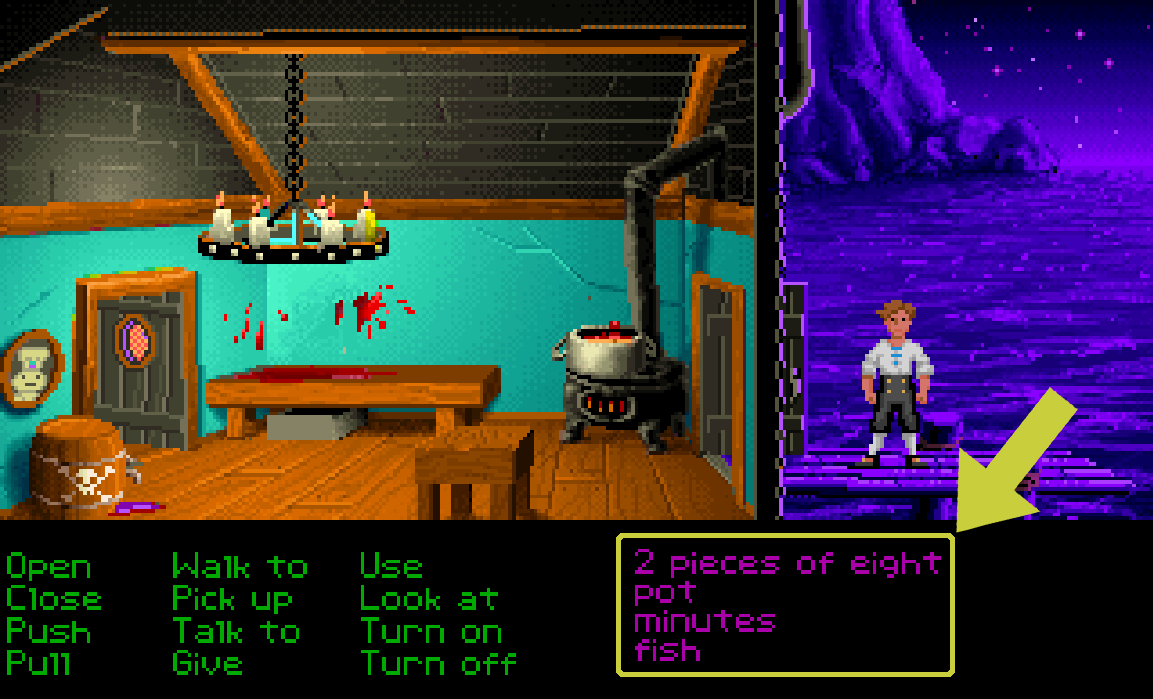
\includegraphics[width=.8\linewidth]{img/I-TSoMI.png}
\caption{The list of items in player's inventory highlighted with purple colour is located in the lower right side of the screen.}
\label{fig:I-TSoMI}
\end{figure}

The inventory in \textit{Beneath the Steel Sky} is slightly hidden. The player must move the mouse cursor to the top of the screen to make the inventory panel slide down. Following this, the player can see the icons of all items in the inventory as well as their names when the mouse hovers over an icon as seen in Figure \ref{fig:I-BaSS1}. To see a longer description, the player has to click on the item with the left mouse button, which is depicted in Figure \ref{fig:I-BaSS2}. The arrows on both sides of the panel are used to scroll through the inventory if it contains enough items.
\begin{figure}[H]
\centering
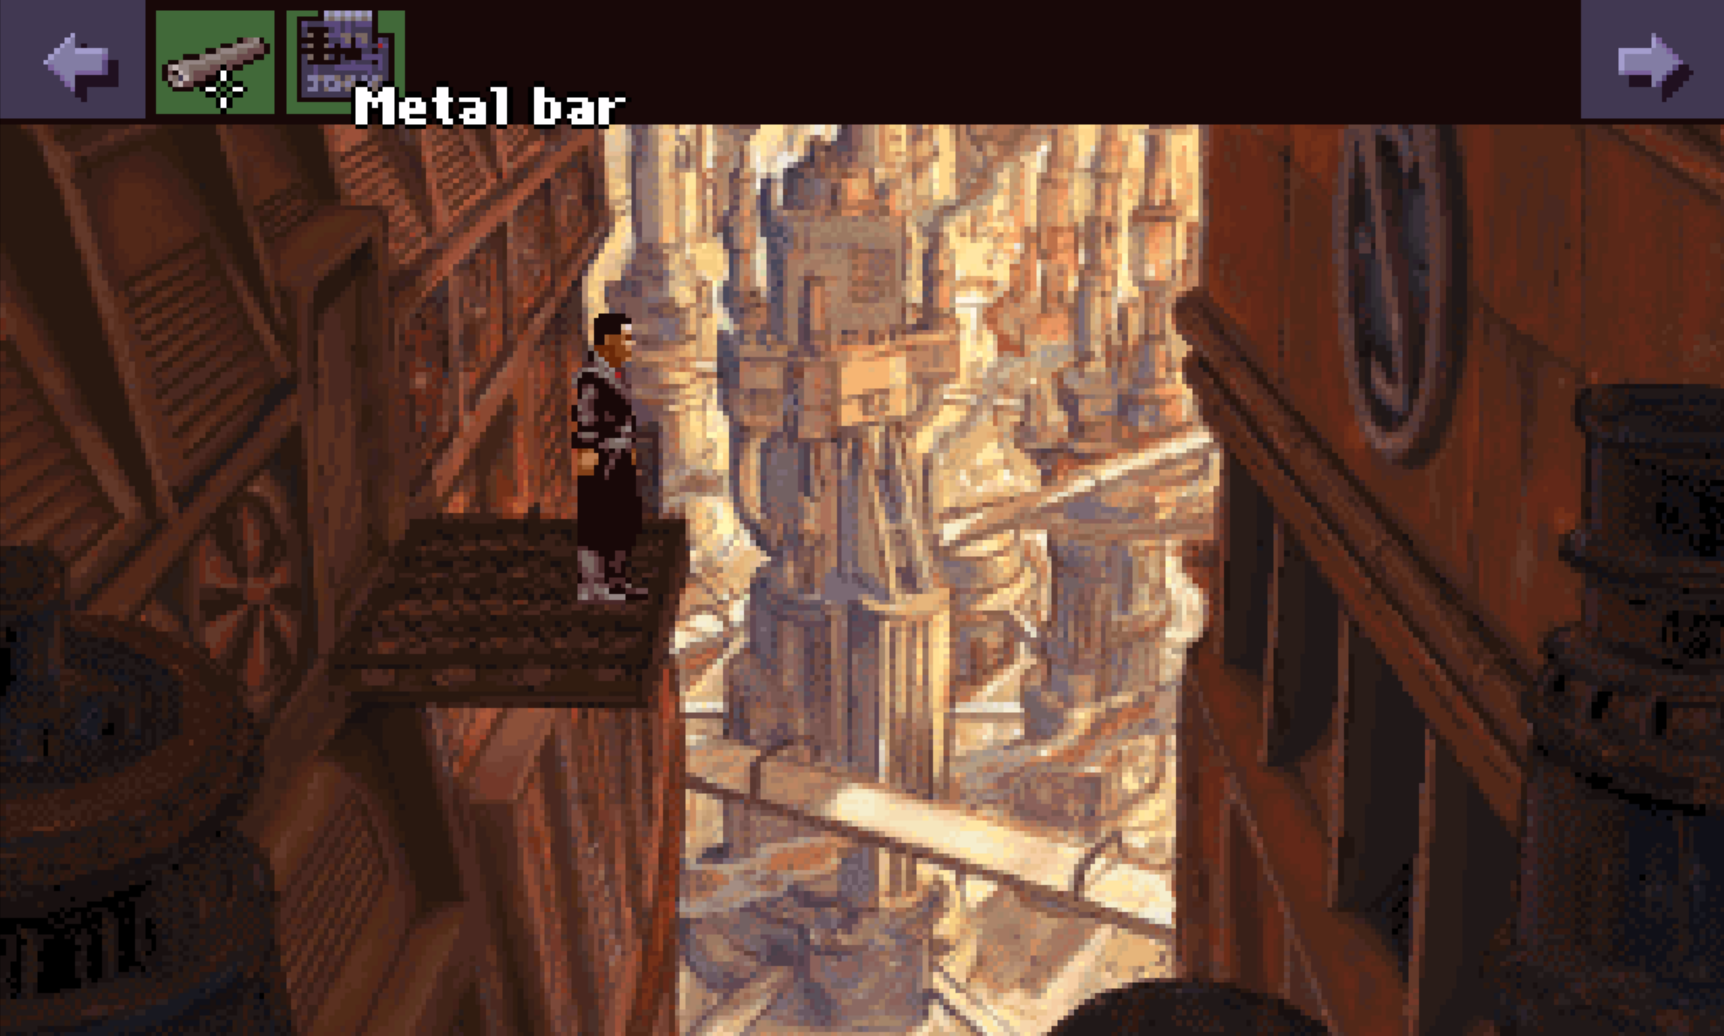
\includegraphics[width=.8\linewidth]{img/I-BaSS1.png}
\caption{In the upper part of the image there is a panel with the inventory. A mouse cursor is hovering over an item and its name is displayed next to the cursor.}
\label{fig:I-BaSS1}
\end{figure}

\begin{figure}[H]
\centering
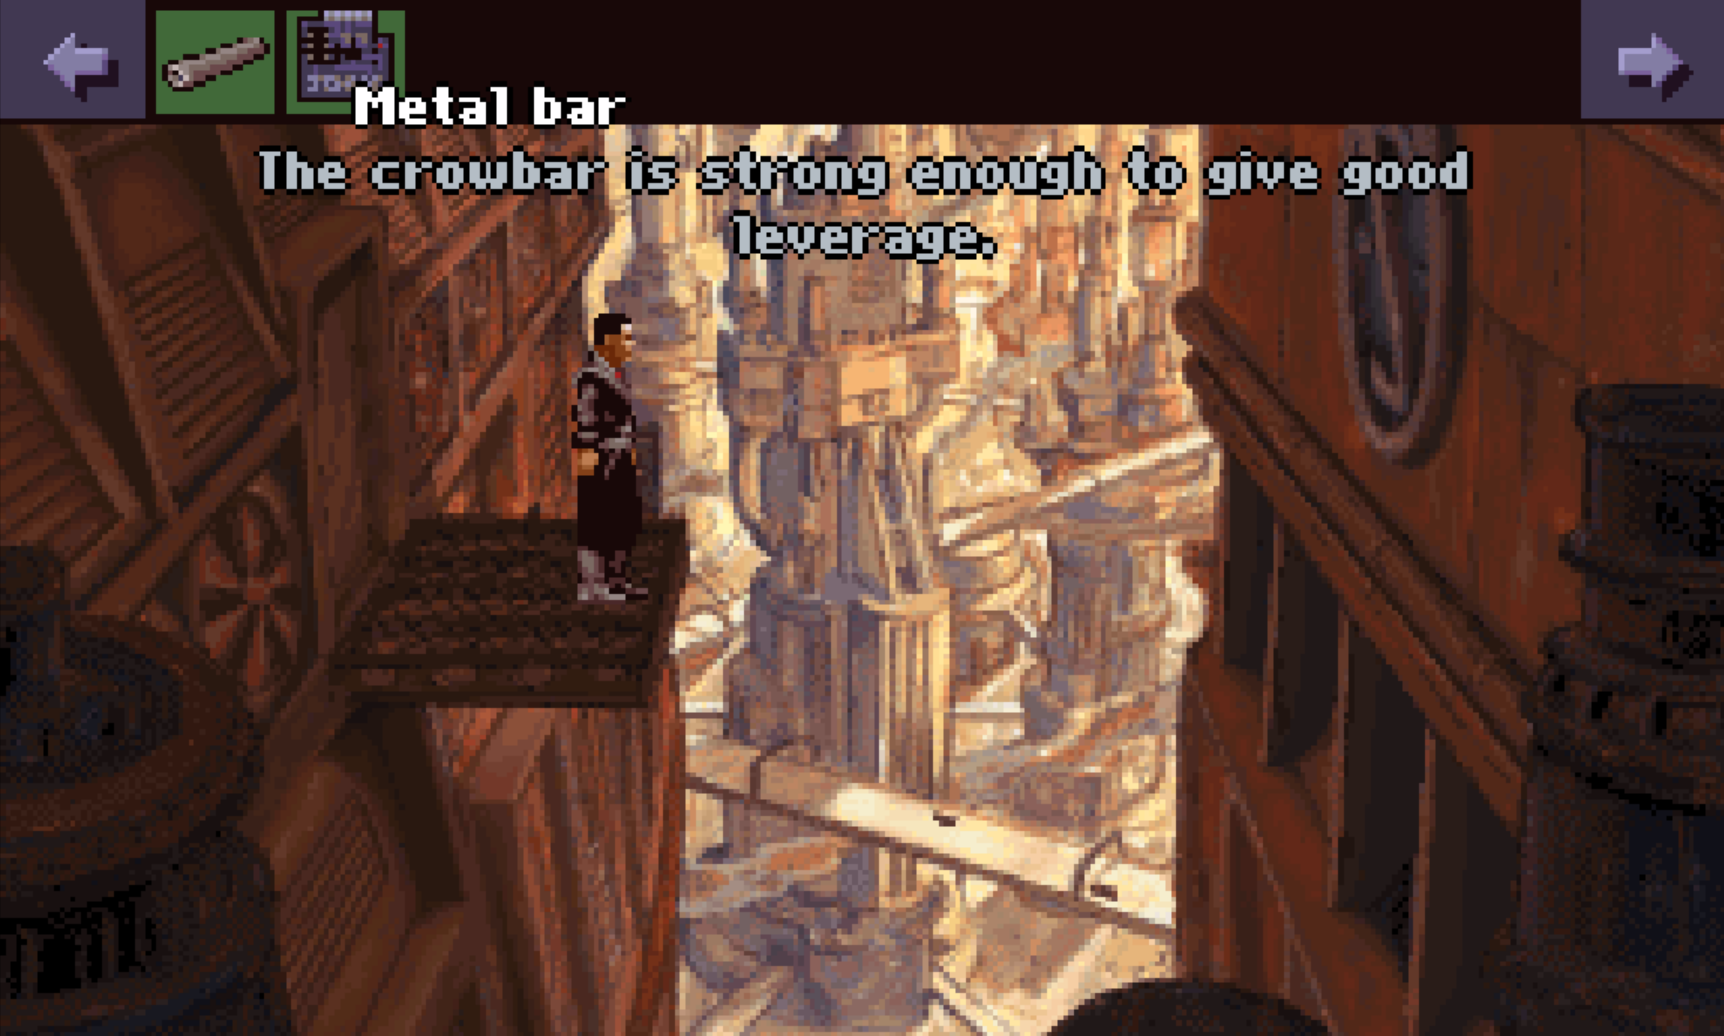
\includegraphics[width=.8\linewidth]{img/I-BaSS2.png}
\caption{In the upper part of the image there is a panel with the inventory. A name of an item in the inventory together with its description is displayed.}
\label{fig:I-BaSS2}
\end{figure}

Other games hide the inventory entirely through a pop-up window. In \textit{Fran Bow}, the inventory can be accessed by clicking on an icon of a purse in the lower left corner of the screen. A panel appears with icons of items. In Figure \ref{fig:I-FranBow}, there is an inventory containing various items.
\begin{figure}[H]
\centering
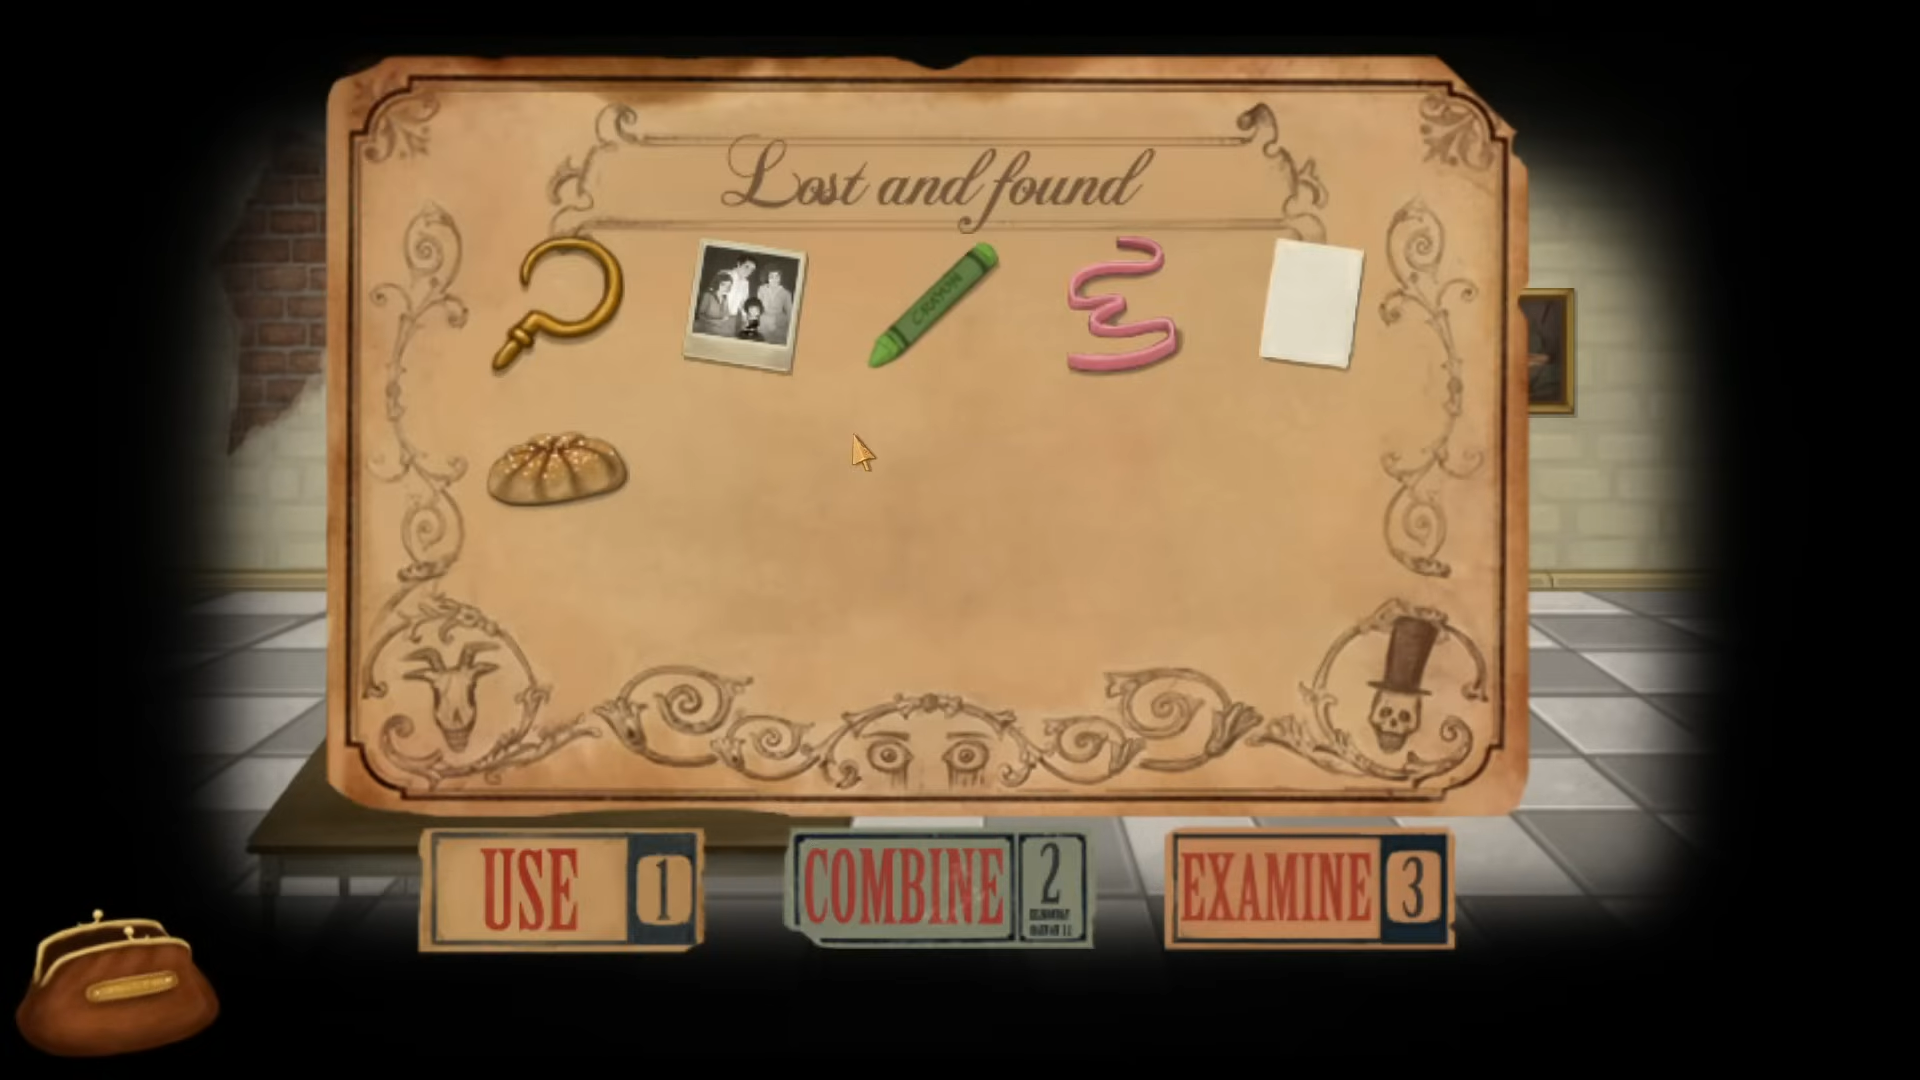
\includegraphics[width=.8\linewidth]{img/I-FB.png}
\caption{In the bottom left corner, there is a brown purse. The inventory in the middle of the screen is a big panel. It contains icons of items the player has collected.}
\label{fig:I-FranBow}
\end{figure}
 
\subsection{Commands}
\label{sec:Commands}
The defining feature of every video game is the ability to engage with this medium. In 2D point-and-click adventure games, the player also has the ability to interact with the world. These commands are executed in a variety of ways.

\subsubsection{Command system}
One of the main ways players can engage with the world is a \textit{command panel}, which is typical of games from the golden era of 2D point-and-click adventure games. A \textit{command panel} consists of a variety of verbs, as seen in Figure \ref{fig:C-TSoMI}. These commands are very contextual--typically, if the player selects a command from the panel and hovers over an object on the screen, a short sentence will be created in the upper part of the panel (\textit{The Secret of Monkey Island}) or above the mouse cursor (\textit{Thimbleweed Park}). This provides an indication to the player of what the main character is going to do. In Figure \ref{fig:C-TSoMI}, the command \texttt{Look at} is selected, and then the mouse cursor is placed over a table. This sequence of actions creates the sentence \texttt{"Look at table"}. By following this logic, longer sentences can be obtained if we also take items in the inventory into account.

\begin{figure}[H]
\centering
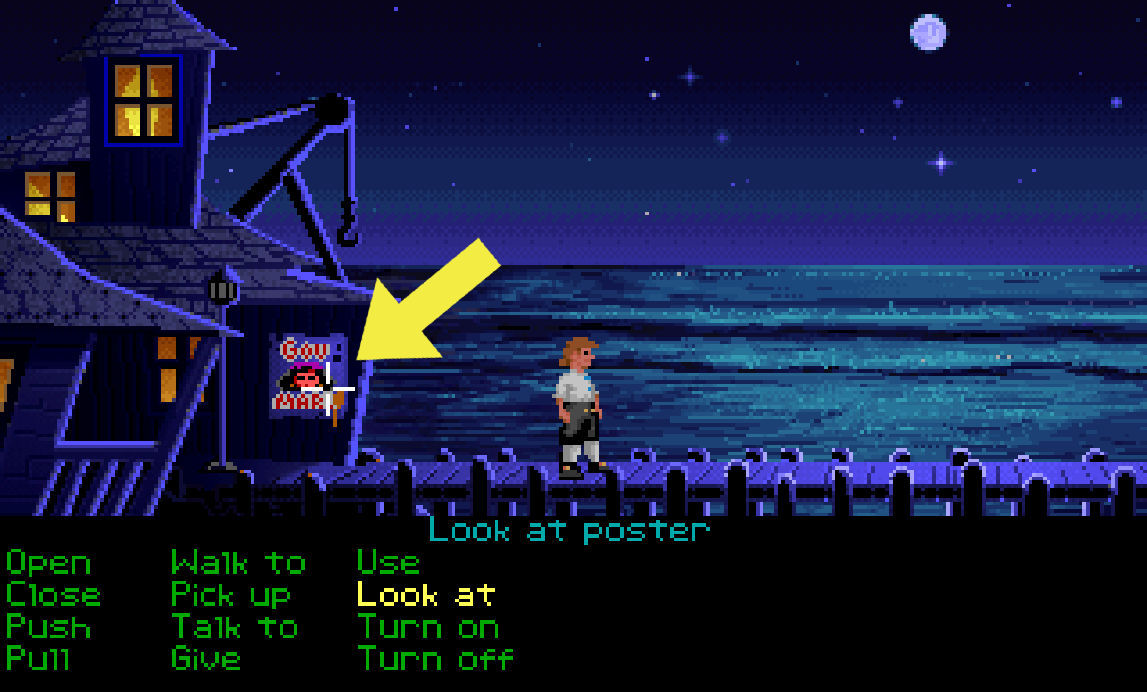
\includegraphics[width=.8\linewidth]{img/C-TSoMI.png}
\caption{In the lower part of the image there is a panel with various commands such as \texttt{Open}, \texttt{Look at}, and \texttt{Use} to interact with the environment. Player's mouse cursor is hovering over a poster and sentence is formed in the upper part of the panel.}
\label{fig:C-TSoMI}
\end{figure}

There are three possible forms of a sentence:
\begin{itemize}
    \item \verb|(verb)| - e.g. \texttt{"Walk to"}
    \item \verb|(verb noun)|, e.g. \texttt{"Look at poster"}
    \item \verb|(verb noun noun)|, e.g. \texttt{\texttt{"Use key with lock"} or "Give ham to dog"}
\end{itemize}
 
For each object in the game, there is a limited number of commands that have a meaningful result. Those that do not make sense for the given object result in the straightforward response something along the lines of \texttt{"That doesn't seem to work."} Then there are some that result in a humorous response, but do not help to progress the story either. And finally, certain panel actions help the player obtain a piece of information (\texttt{Look at}), change the state of an object (\texttt{Open}, \texttt{Push}, etc.), let them talk to an NPC (\texttt{Talk to}), or let them obtain or remove an item from the inventory (\texttt{Pick up} and \texttt{Give}).

\subsubsection{Mouse}
Some games are primarily controlled by the mouse without the need for a panel of actions. Typically, the player clicks on an object with the mouse, and the game decides what to do based on the context. When hovering the mouse cursor over an object, a short text will pop up describing what that object is.

Left - look at
For example, in \textit{Beneath the Steel Sky} when clicking with the right mouse button on an interactable object in the environment, the main character Foster will either pick it up or use it in some way (or talk to an NPC if that object was one). The same action with the left mouse button will result in the main character commenting about (e.g. describing) that object. If the player decides to use an item on an object, they must grab an icon using the right mouse button and then lead the item to the location of the object. This action is captured in Figure \ref{fig:C-BaSS}. Finally, if the player clicks on an empty spot that the main character can reach using either of the mouse buttons, Foster will move there. Overall, the game decides what the action will lead to.

\begin{figure}[H]
\centering
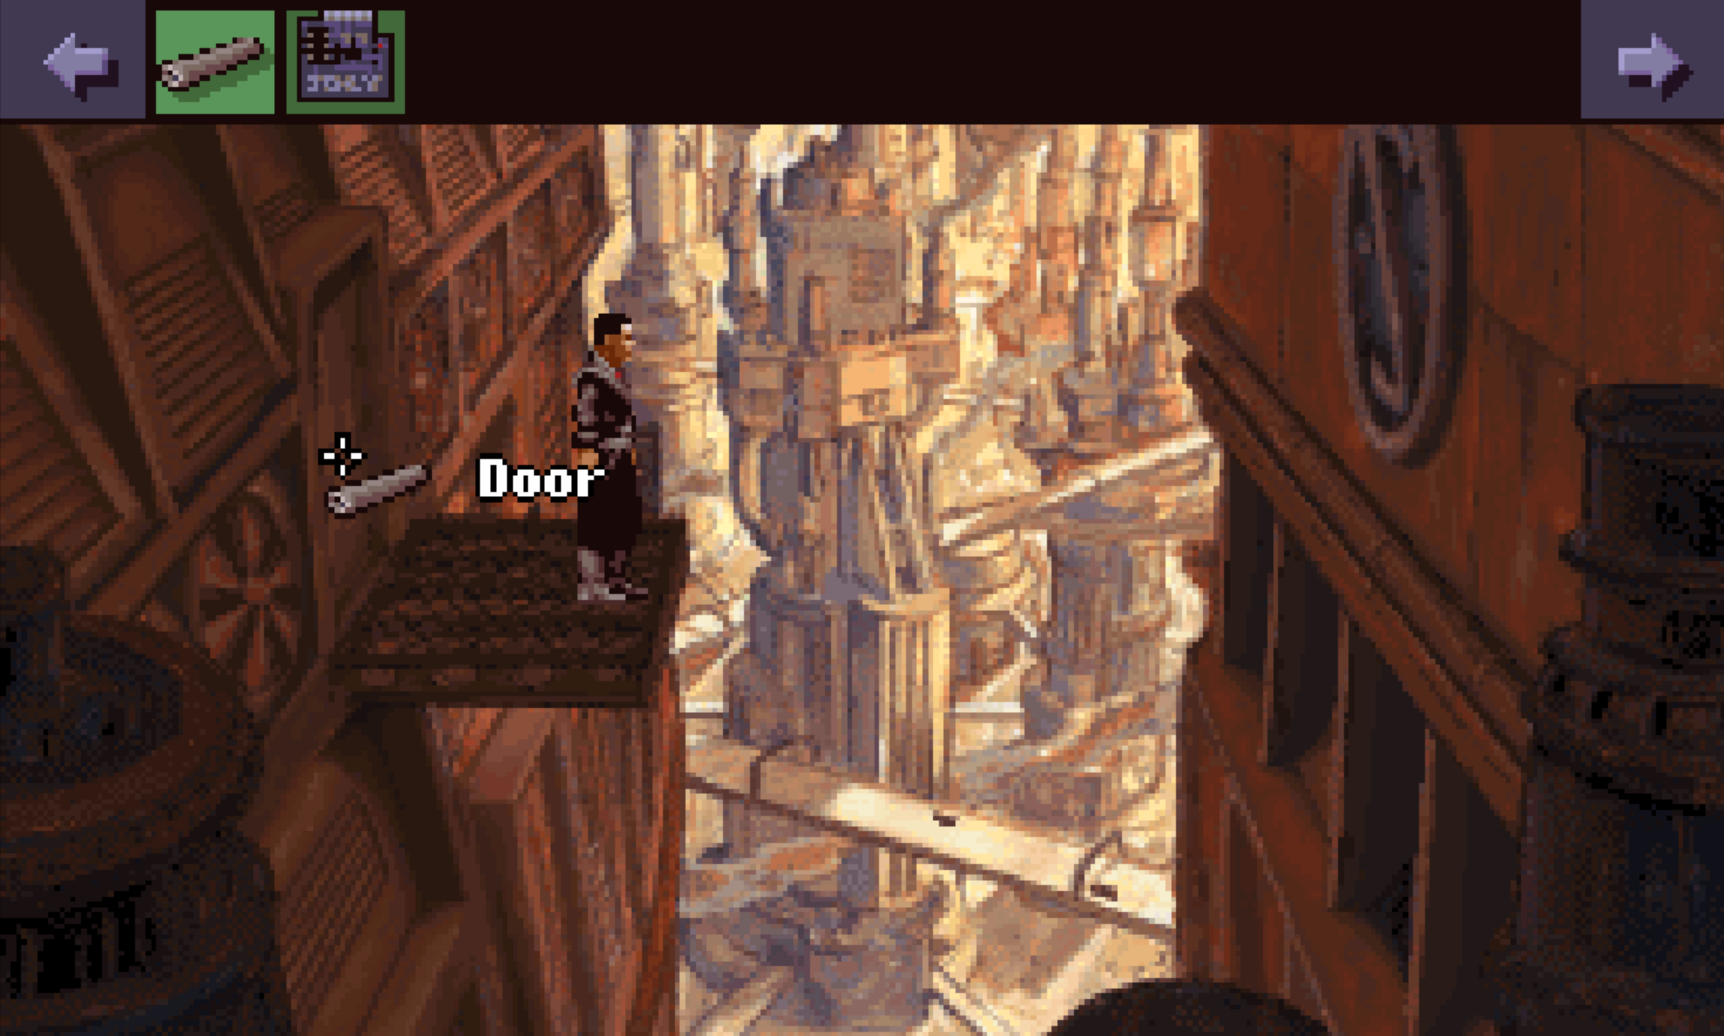
\includegraphics[width=.8\linewidth]{img/C-BaSS.png}
\caption{In the upper part of the image there is a panel with his inventory. A mouse cursor is located on an object (a door) while holding another object (a metal bar) from the inventory.}
\label{fig:C-BaSS}
\end{figure}

\subsubsection{Combination}
Some games combine these two methods like \textit{Fran Bow}. Although the game uses commands, the number of them is limited to three. However, they are much more versatile. When an item is selected and \texttt{Examine} is pressed, the main character Fran Bow says something about the item. In addition, there is a \texttt{Combine} button which allows the player to choose two items and create a new one in their place within the inventory. Finally, the third button with the \texttt{Use} label is a bit more versatile. Depending on the item, the player can either inspect the item closer and interact with it (e.g. unlocking a locked box and finding hidden items), or use the item outside of the inventory (e.g. giving an item to an NPC). At the bottom of the screen, a short sentence is created according to what the player will do as seen in Figure \ref{fig:C-FranBow} . 

In addition to the panel actions, the player can use the mouse. For example, talking to NPCs is done only by clicking the left mouse button, so no command button is necessary. 
\begin{figure}[H]
\centering
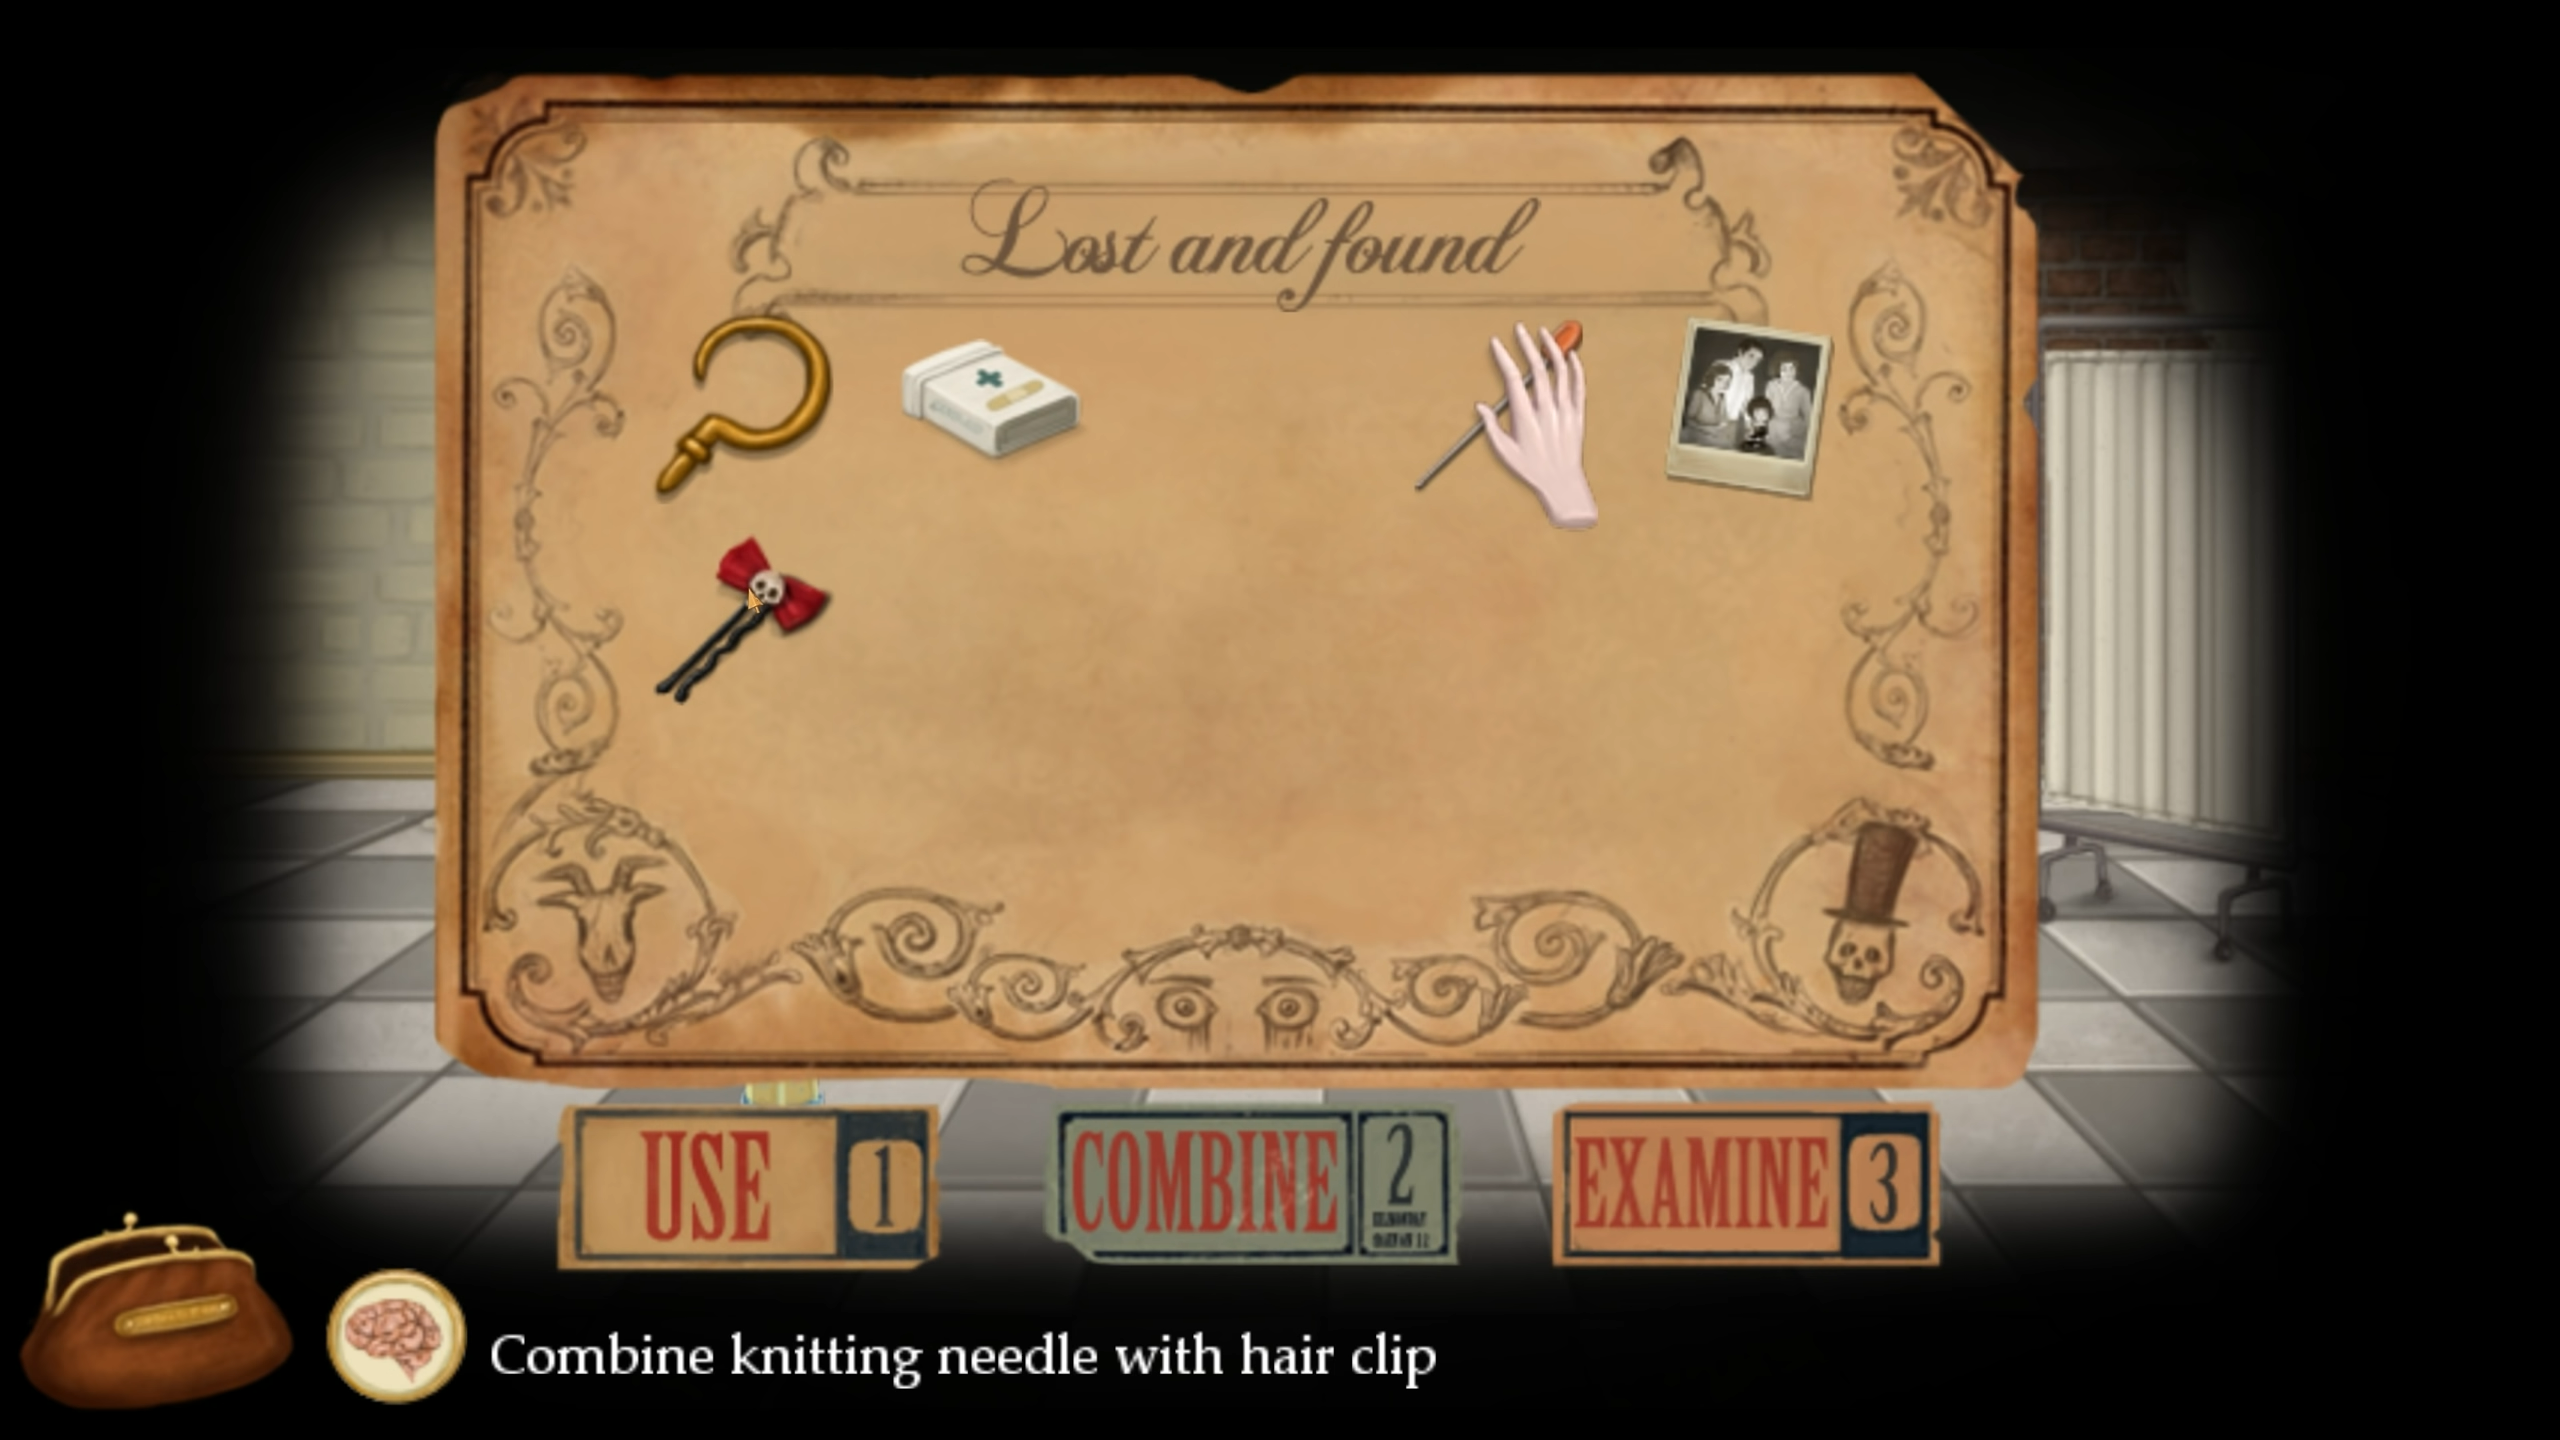
\includegraphics[width=.8\linewidth]{img/Fran_Bow.png}
\caption{Below the inventory there are three action buttons for player to use. At the very bottom there is a sentence describing the action the player is going to take.}
\label{fig:C-FranBow}
\end{figure}

\subsection{Character movement}
\label{sec:Character movement}A typical way to control movement is by clicking on a location in the environment, which prompts the character to find the shortest path and move there.  As outlined in the previous section, the main two ways of character movement either involve or do not involve the use of a command button.

\subsubsection{Command button}
The character movement in \textit{The Secret of Monkey Island} is a prime example of this type of control. To move the character to another position, one must select the \texttt{Walk to} button and then click on a point in the environment that is not occupied by any object as seen in Figure \ref{fig:M-TSoMI}. In case an object stands in that place, the character will just walk to the object without interacting with it.

\begin{figure}[H]
\centering
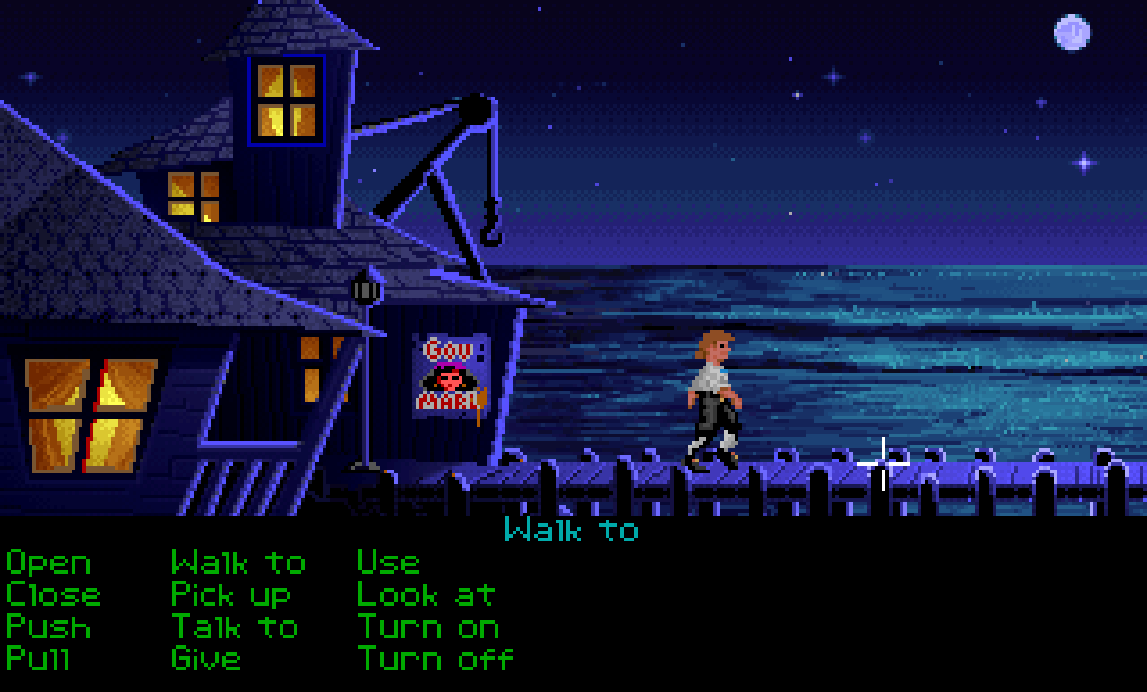
\includegraphics[width=.8\linewidth]{img/W-TSoMI.png}
\caption{A mouse cursor is hovering over a pier while the main character is walking to that point.}
\label{fig:M-TSoMI}
\end{figure}

\subsubsection{Mouse only}
To move the character to another position, it is sufficient to click on a point in the environment with a mouse that is not occupied by any object. If a point occupied by an object is selected, the main character will not only walk to the point but will also interact with it as seen in Figure \ref{fig:M-BaSS}.

\begin{figure}[H]
\centering
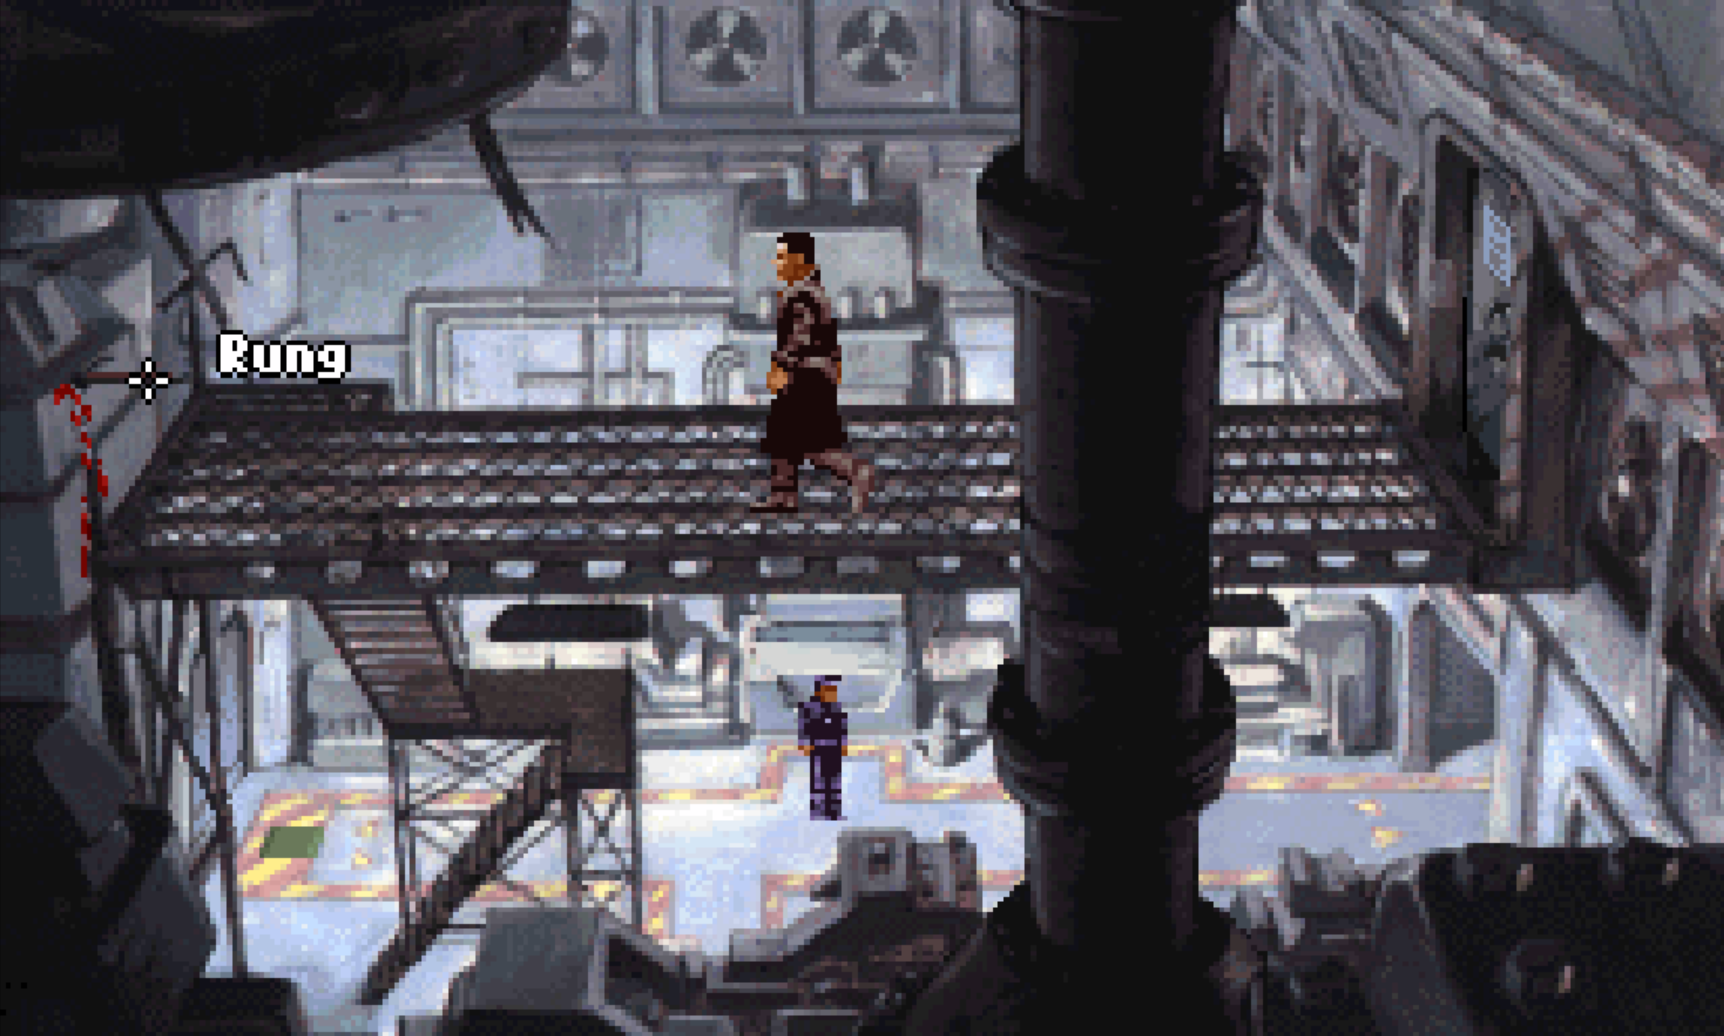
\includegraphics[width=.8\linewidth]{img/M-BaSS.png}
\caption{A mouse cursor is located on an object (a rung) while the main character is walking to the object.}
\label{fig:M-BaSS}
\end{figure}

\subsection{Dialogue}
\label{sec:Dialogue}Dialogues are a very important part of a 2D point-and-click game. In some examples, it is more advanced, with many options to choose from (\textit{The Secret of Monkey Island}), and in others its structure is more simple (\textit{Fran Bow}).  

To initialize a dialogue with an NPC in \textit{The Secret of Monkey Island}, the player must first enter \textit{dialogue mode} by selecting the Talk to command button and afterwards clicking on them, observed in Figure \ref{fig:D-TSoMI0}. When done so, the dialogue initializes, and some features, such as the inventory, are inaccessible. Instead, the player can choose an option on how to respond to the NPC as seen in Figure \ref{fig:D-TSoMI1}. By selecting the option, the player responds, and the dialogue continues until the player has the option to choose an answer again. Typically, subtitles are used to make the dialogue more accessible and understandable even with limited audio, this can be observed in Figure \ref{fig:D-TSoMI2}. To exit \textit{dialogue mode}, a specific option must be selected, and the player is back in \textit{gameplay mode}.
\todo{divide it more between the pictures?}

\begin{figure}[H]
\centering
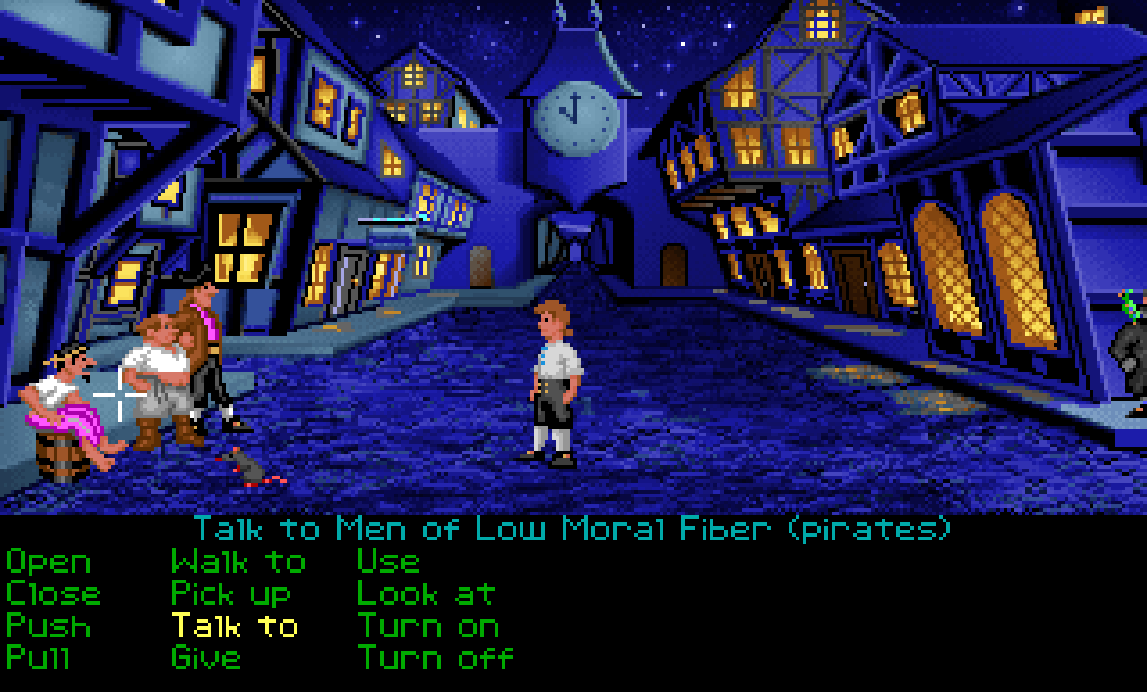
\includegraphics[width=.8\linewidth]{img/D-TSoMI0.png}
\caption{The protagonist of the story is standing in front of a group of NPCs. In the lower part of the screen, there are multiple lines of text. A mouse cursor is hovering over one of them and is highlighted by yellow colour.}
\label{fig:D-TSoMI0}
\end{figure}

\begin{figure}[H]
\centering
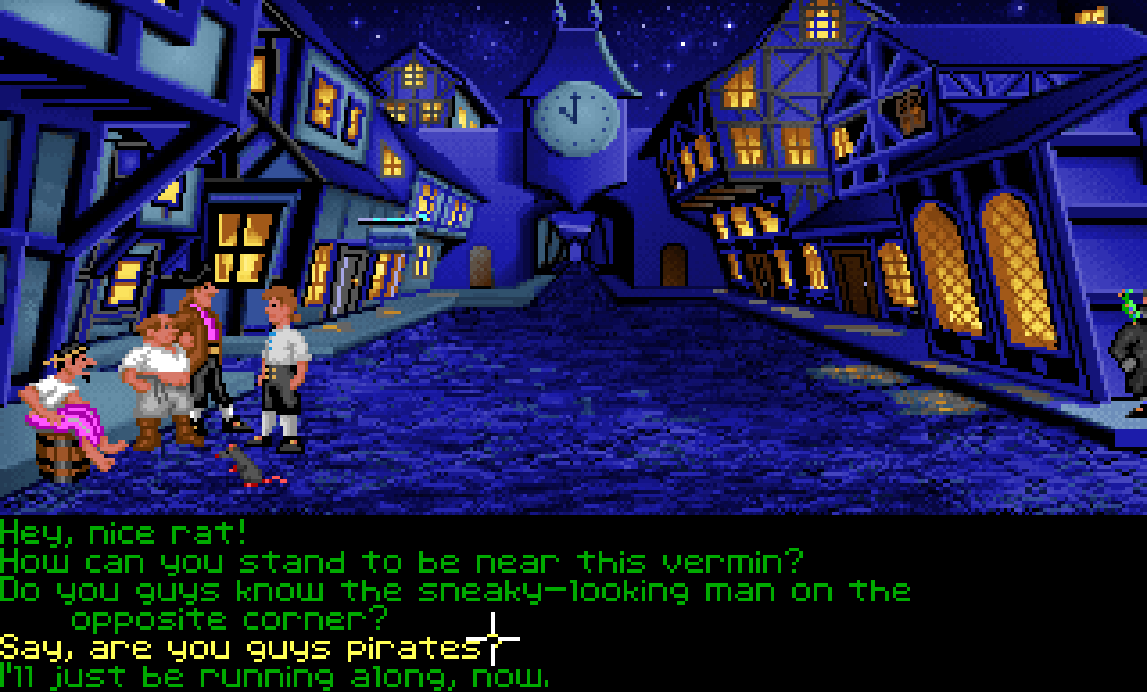
\includegraphics[width=.8\linewidth]{img/D-TSoMI1.png}
\caption{The protagonist of the story is standing in front of a group of NPCs. In the lower part of the screen, there are multiple lines of text. A mouse cursor is hovering over one of them and is highlighted by yellow colour.}
\label{fig:D-TSoMI1}
\end{figure}

\begin{figure}[H]
\centering
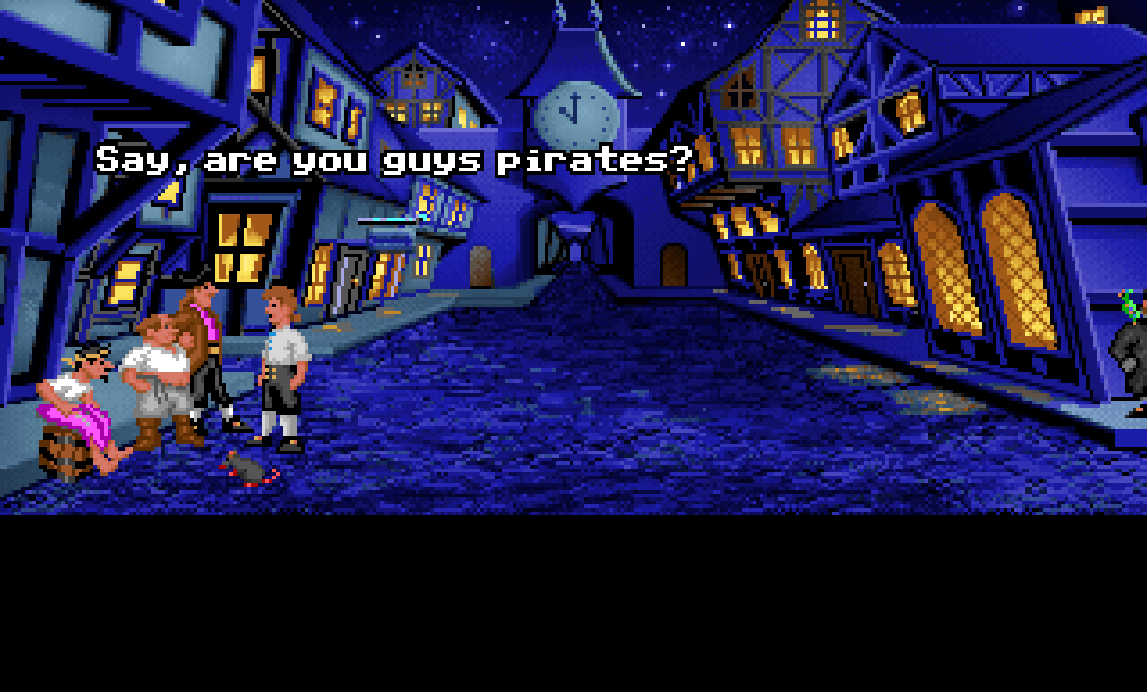
\includegraphics[width=.8\linewidth]{img/D-TSoMI2.png}
\caption{The protagonist of the story is standing in front of a group of NPCs. The panel in the lower part of the screen is empty and there is a line of text hovering above the protagonist.}
\label{fig:D-TSoMI2}
\end{figure}

\textit{Fran Bow} uses a similar approach to NPC dialogue. When the player clicks on an NPC, the dialogue mode is activated. They can interact by choosing one of two options displayed in the bottom panel. In addition, subtitles appear in bubbles above the characters' heads, seen in Figure \ref{fig:D-FranBow}. 

\begin{figure}[H]
\centering
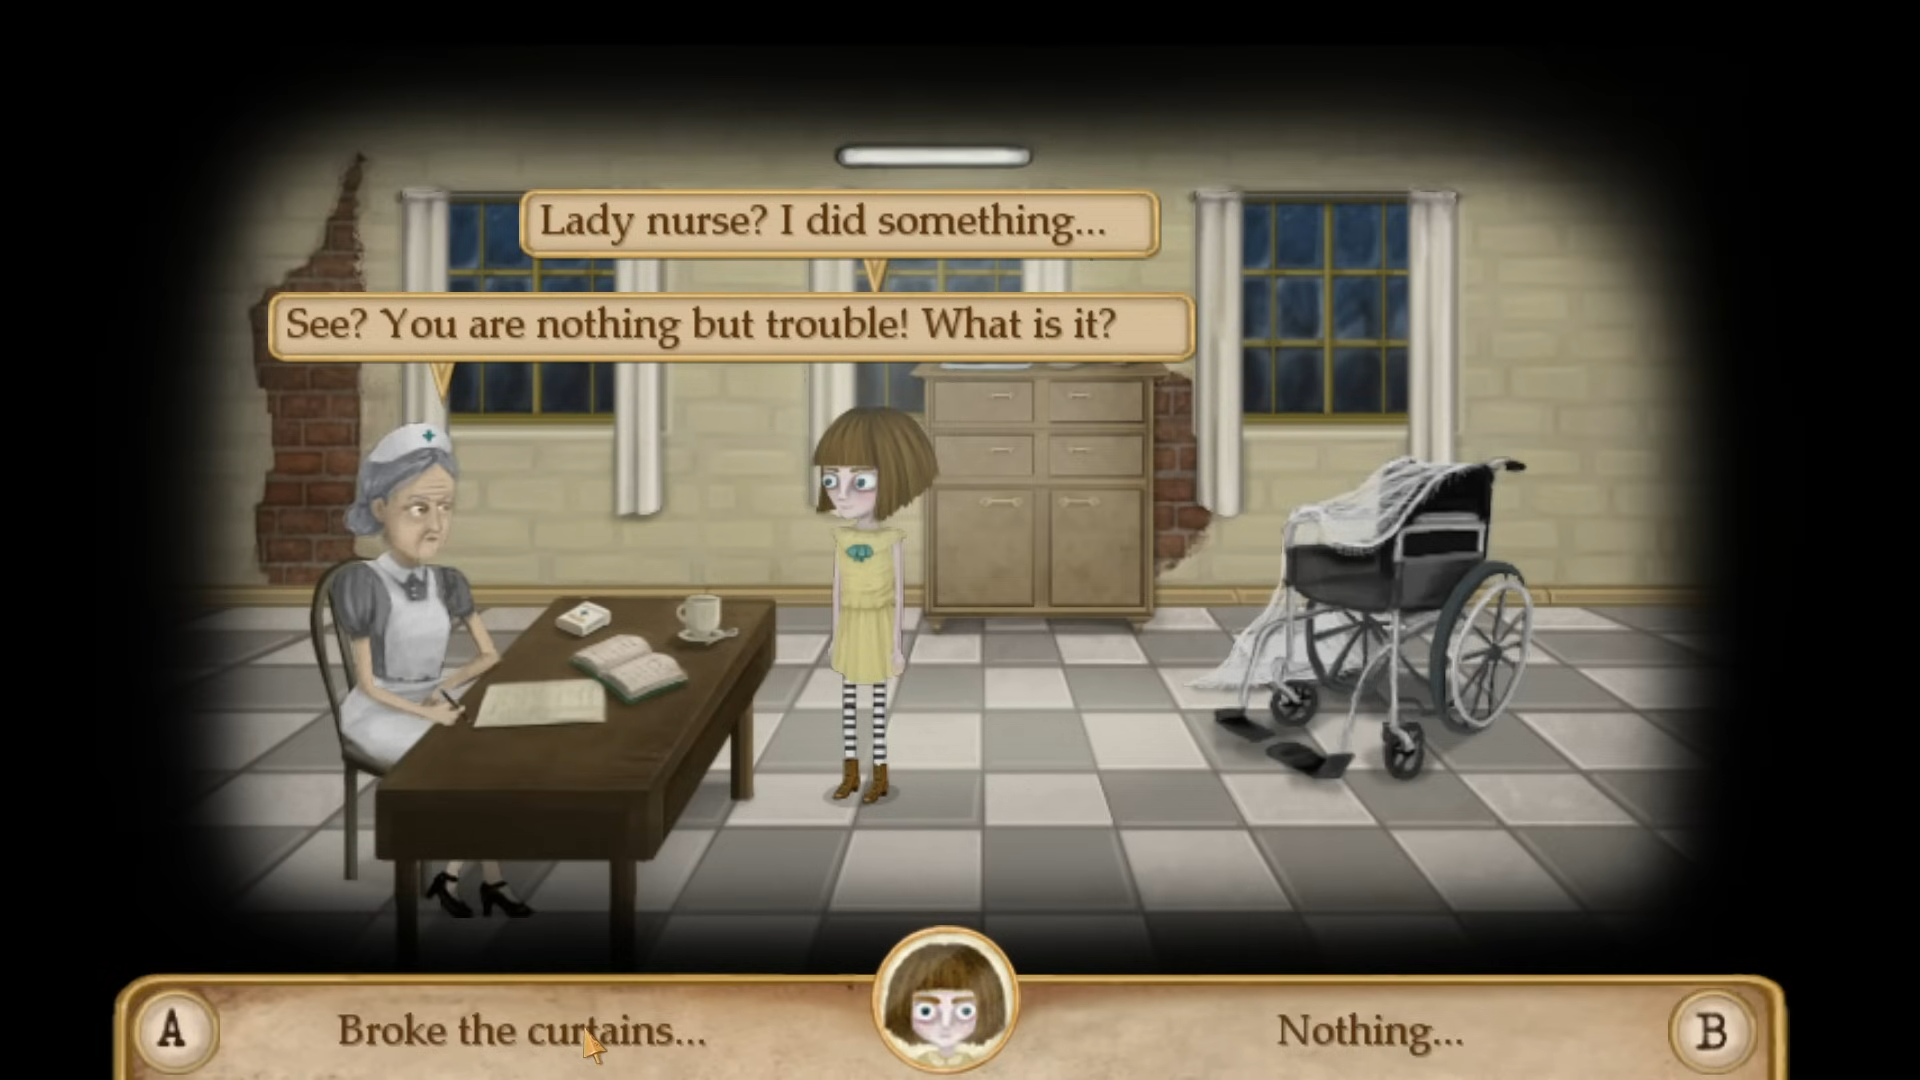
\includegraphics[width=.8\linewidth]{img/D-FB.png}
\caption{The protagonist Fran Bow is talking to an NPC. At the very bottom of the screen, there is a panel with two options of response. Subtitles are located in bubbles above the characters.}
\label{fig:D-FranBow}
\end{figure}

\section{Framework specifications}
Now that the 2D point-and-click adventure games and their common features are understood, the project and its contents can be defined. \todo{too formal? can i use 'we'?}

Our framework will be called \textit{TaleCraft}. Since the goal is to streamline the development of 2D point-and-click adventure games, it should include all the essential mechanics of the genre. Since this thesis aims to create a tool that is both versatile and accessible, \textit{TaleCraft} will provide core systems such as movement, dialogue, and inventory management. It will also allow developers to customize these elements to fit their artistic and narrative vision. To demonstrate its functionality and ease of use, a prototype game will be developed using the framework. 

\subsection{General features}
Since this project aims to simplify game creation, it should offer multiple implementation options for each feature to support a wide range of unique games and ideas. In Section \hyperref[sec:Common features]\{1.2\}, several point-and-click adventure games were introduced. Based on their common features, we will outline what the framework will implement. 

\subsubsection{Inventory}
The inventory can be hidden or visible throughout the game. It can consist of icons or names of items, and there are various options to display the inventory. The goal is to make the process of designing an inventory simple with a variety of options.

\subsubsection{Commands}
As seen in Section\hyperref[sec:Commands]{1.2.2}, here are two main approaches on how to control the actions of a character in a point-and-click game. The goal is to design a system where the creation of the game is simple and versatile so that a developer has the option to combine the two methods in a variety of ways.

\subsubsection{Character movement}
As seen in Section \hyperref[sec:Character movement]{1.2.3} the character movement is primarily controlled through the mouse. Other genres allow the player to move around the environment using arrow keys or WASD keys. This is a very uncommon approach in the point-and-click genre. The name of the genre itself contains the words 'point' and 'click'. I feel like by including the option to move the character using keys, it would break the essence of the genre. This is why I will not include this option and stick to the mouse control presented in Section \hyperref[sec:Character movement]{1.2.3}. This includes path finding in the environment and between various obstacles.

\subsubsection{Dialogue}
The dialogue in the genre of point-and-click adventure games is fairly straightforward. It consists of subtitles that can be displayed anywhere on the screen and a set of dialogue options to choose from.

\subsection{Technology}
To develop our game, we will use the Unity editor where we can do tasks like creating tracks, designing the UI, etc. Microsoft Visual Studio will be used for writing C# scripts. 


\section{Games}
\todo{throw out!}
\subsection{The Secret of Monkey Island (1990)}
Released in 1990 by Lucasfilm Games, The Secret of Monkey Island is a 2D point-and-click graphic adventure game set in the Caribbean. Our main protagonist is Guybrush Threepwood, an aspiring pirate who embarks on his quest to achieve his dream.
The main character's movement is managed through mouse clicking, a common method in 2D point-and-click games from this era. Other notable features of the game include puzzles, cutscenes, and dialogue trees. 

\subsection{Beneath a Steel Sky (1994)}
Developed by the British studio Revolution Software and launched in 1994, Beneath a Steel Sky is a point-and-click adventure game set in a cyberpunk-inspired dystopian future. The players guide Robert Foster as he uncovers hidden secrets of this foreign world.


\subsection{Fran Bow (2015)}
Created by the Swedish indie studio Killmonday Games, Fran Bow is a 2D point-and-click adventure game with elements of psychological horror. The game is set in 1944 and it tells the story of Fran, a ten-year-old girl suffering from a mental illness after the death of her parents.

The main character's movement is also managed through mouse clicking. The game includes puzzles, cutscenes, and fairly straightforward dialogue trees.

\todo{write how to talk to NPCs}



\subsection{Thimbleweed Park (2017)}
Thimbleweed Park, developed by Terrible Toybox, serves as a spiritual successor to Maniac Mansion (1987) and The Secret of Monkey Island (1990) and is crafted to emulate the visual style and gameplay mechanics of graphic adventure titles from that era. Thimbleweed Park tells the intriguing story of two detectives brought in to investigate a mysterious body discovered in a river near the town. The players switch between five different characters as they enter the dark, satirical, and eccentric world of Thimbleweed Park\cite{Matulef2014}.

\todo{write more describing the game}

\begin{figure}[H]
\centering
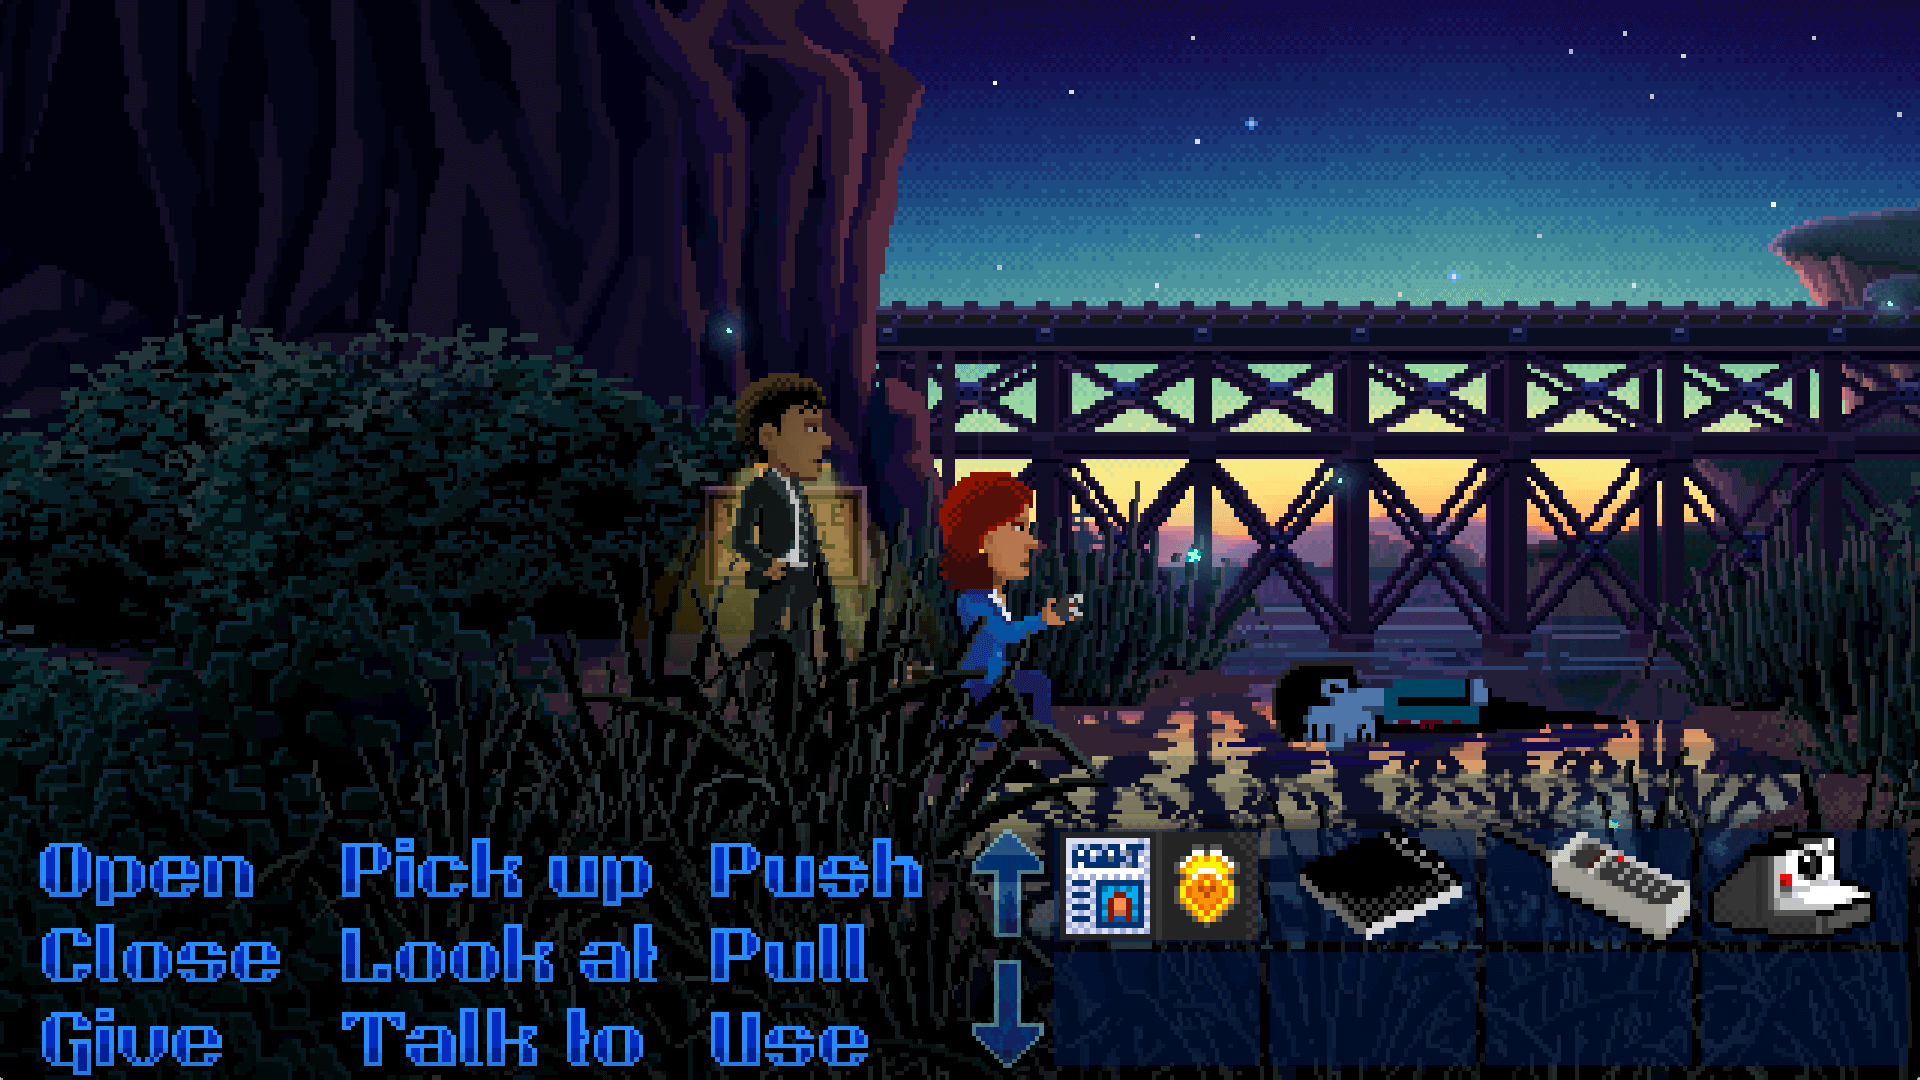
\includegraphics[width=1.\linewidth]{img/TWP.png}
\caption{The player is controlling one of the two FBI agents Angela Ray. She is squatting and taking a picture of a body. In the lower part of the image there is a panel with panel actions such as 'Open', 'Pick up', and 'Talk to'. It also includes a list of items in player's inventory. Its layout is very reminiscent of the one in Figure \ref{fig:TSoMI}. Source: https://store.epicgames.com \cite{epic:TWP}}
\label{fig:TWP}
\end{figure}



\subsection{Return to Monkey Island (2022)}
Return to Monkey Island, created by Terrible Toybox in collaboration with Lucasfilm Games, is a 2D point-and-click adventure game and the sixth entry in the Monkey Island series. The pirate Guybrush Threepwood returns once again to uncover the secret of Monkey Island\cite{McCaffrey2022}.

\todo{write more describing the game. also 0.7 for pics so that they fit on page}

\begin{figure}[H]
\centering
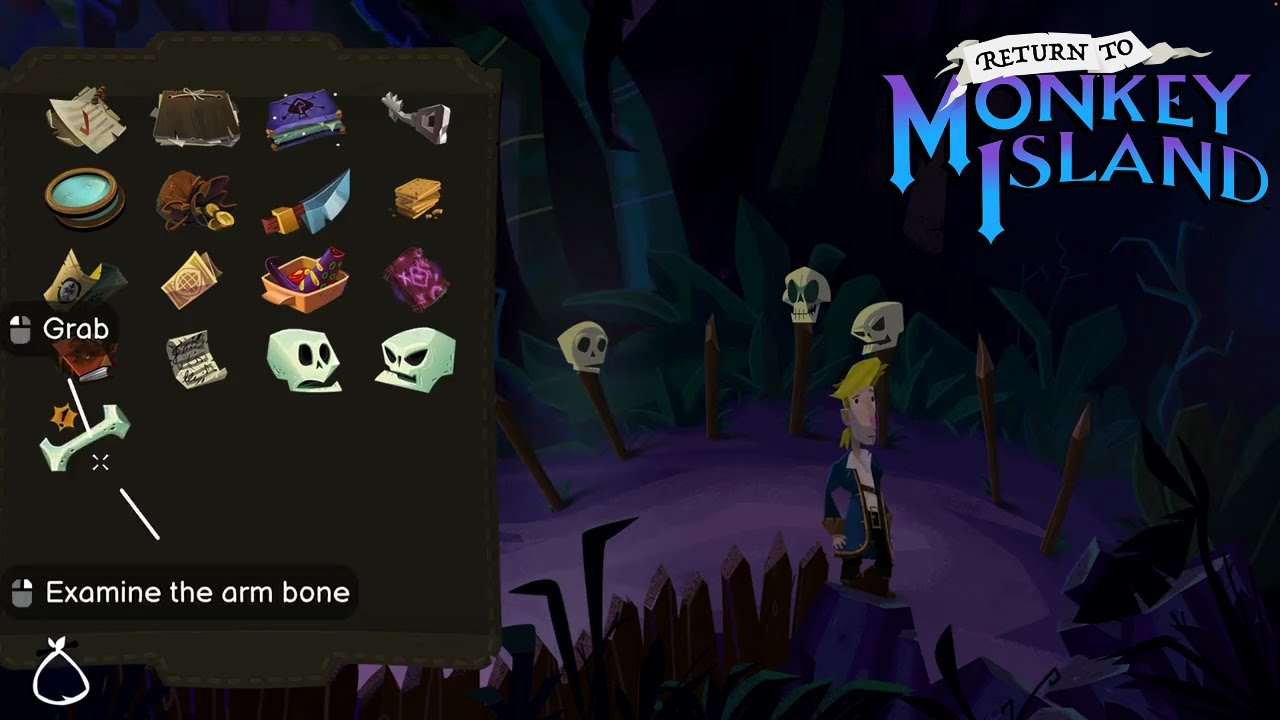
\includegraphics[width=.7\linewidth]{img/RtMI1.png}
\caption{Source:  \cite{}}
\label{fig:RtMI1}
\end{figure}

\begin{figure}[H]
\centering
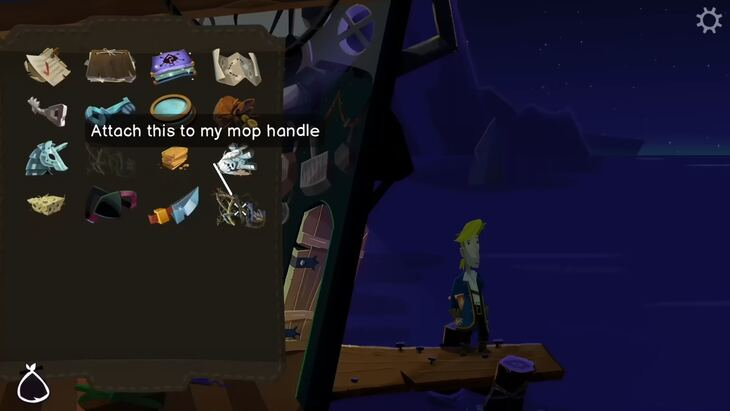
\includegraphics[width=.7\linewidth]{img/RtMI2.png}
\caption{Source:  \cite{}}
\label{fig:RtMI2}
\end{figure}
